\pagenumbering{arabic}
\section{介绍}
工作场所伤害、疾病和死亡统计数据表明,建筑施工中的职业健康
和安全 (OHS) 仍然是一个全球性问题。超过三分之一 (36\%) 的美国工作场
所的死亡事故发生在建筑业。同样,芬兰的建筑业造成了四分之一的死
亡职业事故。与其他几个行业一样,安全规划在生产规划领域占有关键地
位。然而,在建筑施工行业的安全,安全规划是与工程项目设计及规划阶段分开进行。
尽管高处坠落仍然是建筑工地的一个主要安全风险。但是在大
多数现有项目中,高处坠落保护计划通常要等到施工开始后才会制定。在施
工计划阶段发现和解决安全问题时还会出现其他问题。例如,在建筑工
程项目存在的恶劣天气(气候、独特性)和动态(多种资源、时间限制)条件
下,工人层面的安全交流尤其具有挑战性。以前的几项研究也报告了类似
的问题。

有效的安全规划的主要障碍之一是传统的安全规划仍然主要依赖
纸质的二维图纸和时间表来了解建筑工地的安全装备需求。在防止高处坠落
方面,图 \ref{fig:c1f1} 提出了一个传统的防跌落计划的例子,其中各种防跌落系统已被
标记为不同颜色的建设计划

\begin{figure}[thbp!]
    \centering
    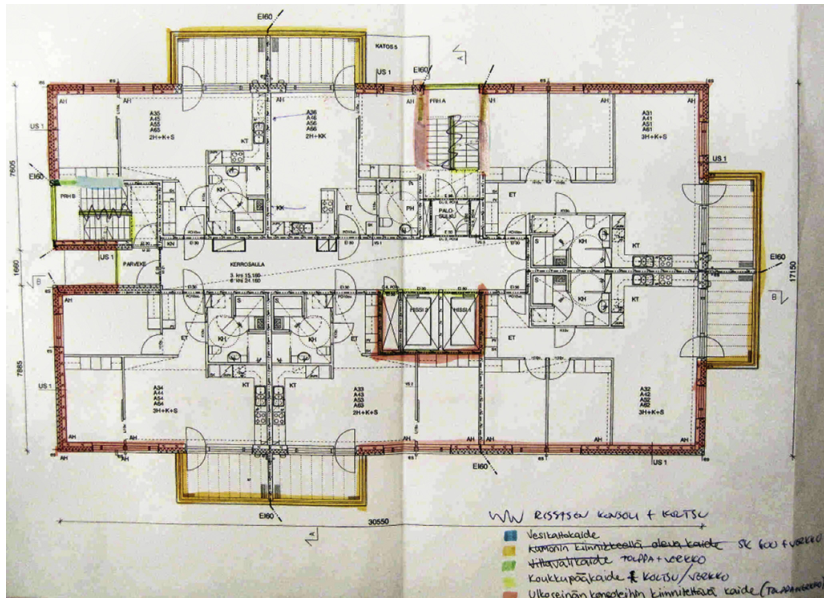
\includegraphics[width=0.8\linewidth]{res/c1f1.png}
    \caption{传统跌落保护计划的示例}
    \label{fig:c1f1}
    \end{figure}

这样手工的高处坠落危害辨识和计划会导致低效率,其中一些原因是:

\begin{itemize}
    \item 它需要专业的安全工程师根据自己的经验发现潜在的安全隐患并确定安全设备。
    \item 许多安全问题是隐含的,因为建筑计划中没有标明部分完整的条件。
    \item 建设项目的动态性导致了安全需求的变化。基于静态图纸,很难确定不同施工阶段、进度表的潜在跌落危险。
    \item 施工进度会因天气、材料交付等因素而发生变化,导致安全计划发生变化。每次更改时间表都要更新安全计划,这既费时又费力。
    \item 举例来说,与小的孔洞能给足部造成伤害相比,人会更容易发现他们自己即将在边缘跌落到低处。这些漏洞很难或从未在纸质计划中绘制,因此可能永远不会被发现,即使是专家。
\end{itemize}   

目前用于处理和报告建筑项目安全和健康相关问题的方法效率低下。
新型技术可以协助施工安全专家更容易识别和解决安全隐患,同时解决施工现
场条件的复杂性和动态性,从而可以更安全的施工和更少的努力。

建筑信息模型 (BIM) 是一种对设备的物理和功能特性的数字表示建筑
信息模型。BIM 是一种共享的知识资源,用于获取有关设施的信息,这
些信息为设施在其生命周期中的决策提供了可靠的基础;定义为从最初构
想到拆除的存在。建筑信息模型 (BIM) 在建筑/工程/建筑 (AEC) 和设施
管理 (FM) 行业的不断推广,正在改变人们对待安全的方式。建筑信息
模型 (BIM) 在施工作业计划和管理以及安全管理中的应用正在迅速增加。
一个出发点是在建筑设计和工程阶段的早期强调安全方面。 Zhang et al 同时指出,
建筑业需要解决目前使用的纸张和人工安全程序效率低下的问题。

基于 BIM 的方法正被应用于建筑设计和规划。在工地安全管理和监
督方面也越来越多地实施这些措施。人工安全检查通常遵循以下程
序:
\begin{itemize}
    \item 使用建造工程进度表,以确定建造工程的施工动作、次序或工程任务项目的空间布局
    \item 确定造成安全隐患的临时条件
    \item 规划纠正措施以消除安全隐患
    \item 将这些纠正措施整合到方案中
\end{itemize}

然而,人类的认知技能仅限于心理模拟。
复杂的环境表明,一个更加积极的、基于仿真的方法和使用预定义的模式检查
可以大大加强这一系列活动的有效性。
正如 Kiviniemi 所说,只有拥有一套完整的方法才能成功地提供所有领域的能力。

在前人研究成果的基础上,本研究旨在开发一个基于 BIM 的跌落危
险自动识别与规划工具,该工具

\begin{itemize}
    \item 基于施工进度动态识别潜在跌落危险
    \item 有效协助劳动密集型作业的防跌落系统的建模与规划任务
    \item 通过可视化潜在危险提高工人的安全意识
\end{itemize}

本案例研究还旨在评估自动化安全代码检
查和规划的可能性、好处和开发需求。此外,我们还研究了开发的基于
BIM 的原型工具的可用性和成熟性,该工具用于支持建筑施工项目中的
预防规划。

本文结构如下:第一部分对传统的减灾方法和信息建模在施工安全规
划中的应用进行了综述。第二部分介绍了已开发的安全规则检验原型及
其计算方法。第三部分介绍了原型在两个案例研究中的应用。在第一个案例
研究中,讨论了跌落保护系统的人工建模和自动建模,并对设计方案与
实际情况进行了比较。在第二个案例中,以施工进度计划为例,说明了
样机产生的跌落危险检测和防护的动态特性。第四部分比较了几种 BIM 在
建筑安全规划中的应用。论文的最后一部分对研究结果和贡献进行了总
结和讨论。